\section*{Chapter 4}

\subsection*{Exercise 4.1}
The point $(\theta,\varphi)$ on the bloch sphere represents the state
\begin{align}
     \ket{v}=\cos \frac{\theta}{2}\ket{0}+\sin\frac{\theta}{2}(\cos\varphi+i\sin\varphi)\ket{1}.
\end{align}

For $X$, the eigenvectors and the points on the bloch sphere are:
\begin{align}
    \ket{v_{+1}}=\frac{\ket{0}+\ket{1}}{\sqrt{2}}, (\theta,\varphi)=(\frac{\pi}{2},0),\\
    \ket{v_{-1}}=\frac{\ket{0}-\ket{1}}{\sqrt{2}}, (\theta,\varphi)=(\frac{\pi}{2},\pi).
\end{align}

For $Y$, the eigenvectors and the points on the bloch sphere are:
\begin{align}
    &\ket{v_{+1}}=\frac{\ket{0}+i\ket{1}}{\sqrt{2}}, (\theta,\varphi)=(\frac{\pi}{2},\frac{\pi}{2}),\\
    &\ket{v_{-1}}=\frac{\ket{0}-i\ket{1}}{\sqrt{2}}, (\theta,\varphi)=(\frac{\pi}{2},\frac{3\pi}{2}).
\end{align}

For $Z$, the eigenvectors and the points on the bloch sphere are:
\begin{align}
    &\ket{v_{+1}}=\ket{0}, (\theta,\varphi)=(0,0),\\
    &\ket{v_{-1}}=\ket{1},
    (\theta,\varphi)=(\pi,0).
\end{align}


\subsection*{Exercise 4.2}

Because $A^2 = I$, then for any of $A$'s eigenvalue $v$ and eigenvector $\ket{v}$, we have:
\begin{align}
    A^2\ket{v_i}=A(v_i\ket{v_i})=v_i^2\ket{v_i}=\ket{v_i}.
\end{align}

So $v_i=\pm 1$. Therefore, $\cos(v_i x)=\cos(x),\sin(v_i x)=v_i \sin(x)$

Then we have:
\begin{align}
\exp(iAx)&=\exp\left(i\sum_i v_i \ket{v_i}\bra{v_i}x\right)\\
&=\sum_i \exp(iv_i x) \ket{v_i}\bra{v_i}\\
&=\sum_i(\cos(v_i x)+i\sin(v_i x))\ket{v_i}\bra{v_i}\\
&=\sum_i(\cos(x)+i\sin( x)v_i)\ket{v_i}\bra{v_i}\\
&=\cos(x)I+i\sin(x)A.
\end{align}

\subsection*{Exercise 4.3}

\begin{align}
    R_z&(\pi/4)=\begin{pmatrix}e^{-i\pi/8} & 0 \\0 & e^{i\pi/8} \end{pmatrix},\\
    T&=\begin{pmatrix}1 & 0 \\0 & e^{i\pi/4} \end{pmatrix}=e^{i\pi/8}R_z(\pi/4).
\end{align}

\subsection*{Exercise 4.4}
\begin{align}
    R_z(\pi/2)R_x(\pi/2)R_z(\pi/2)&=
    \begin{pmatrix}e^{-i\pi/4} & 0 \\0 & e^{i\pi/4}\end{pmatrix}
    \begin{pmatrix}\cos \frac{\pi}{4}& -i\sin\frac{\pi}{4} \\ -i\sin\frac{\pi}{4} & \cos \frac{\pi}{4}\end{pmatrix}
    \begin{pmatrix}e^{-i\pi/4} & 0 \\0 & e^{i\pi/4}\end{pmatrix}\\
    &= \begin{pmatrix}e^{-i\pi/2}\cos \frac{\pi}{4}& -i\sin\frac{\pi}{4} \\ -i\sin\frac{\pi}{4} & e^{i\pi/2}\cos \frac{\pi}{4}\end{pmatrix}\\
    &= \frac{-i}{\sqrt 2}\begin{pmatrix}
    1&1\\1&-1
    \end{pmatrix},
\end{align}
\begin{align}
    H=\frac{1}{\sqrt 2}\begin{pmatrix}
    1&1\\1&-1
    \end{pmatrix}
    =e^{-i\pi/2} R_z(\pi/2)R_x(\pi/2)R_z(\pi/2).
\end{align}

\subsection*{Exercise 4.5}
We have proved the anti-communicator relationship in Chapter 2:
\begin{align}
    \{\sigma_i,\sigma_j\}=2\delta_{ij}I.
\end{align}

Therefore, we have:
\begin{align}
    (\hat n \cdot \vec\sigma)^2&=(n_1\sigma_1+n_2\sigma_2+n_3\sigma_3)^2\\
    &=\sum_i n_i^2\sigma_i^2+n_1n_2(\sigma_1\sigma_2+\sigma_2\sigma_1)+n_2n_3(\sigma_2\sigma_3+\sigma_3\sigma_2)+n_3n_1(\sigma_3\sigma_1+\sigma_1\sigma_3)\\
    &=(n_1^2+n_2^2+n_3^2)I\\
    &=I.
\end{align}

Using Taylor expansion and the equation, we have:
\begin{align}
    R_{\hat n}(\theta)&=\exp(-i\theta\hat n \cdot \vec\sigma/2)\\
    &=1-i\frac{\theta}{2}\hat n\cdot \vec \sigma-\frac{1}{2!}\left(\frac{\theta}{2}\right)^2I+\frac{i}{3!}\left(\frac{\theta}{2}\right)^3\hat n\cdot \vec \sigma+\frac{1}{4!}\left(\frac{\theta}{2}\right)^4I-\cdots\\
    &=\left(1-\frac{1}{2!}\left(\frac{\theta}{2}\right)^2+\frac{1}{4!}\left(\frac{\theta}{2}\right)^4-\frac{1}{6!}\left(\frac{\theta}{2}\right)^6+\cdots\right)I\notag\\
    &-i\left(\frac{\theta}{2}-\frac{i}{3!}\left(\frac{\theta}{2}\right)^3+\frac{i}{5!}\left(\frac{\theta}{2}\right)^5-\frac{i}{7!}\left(\frac{\theta}{2}\right)^7+\cdots\right)\hat n\cdot \vec \sigma\\
    &=\cos\left(\frac{\theta}{2}\right)I-i\sin\left(\frac{\theta}{2}\right)\hat n \cdot \vec \sigma.
\end{align}

\subsection*{Exercise 4.6}

We can first prove that the effect of the rotation $R_x(\theta)$, $R_y(\theta)$ and $R_z(\theta)$ on any state is to rotate it by $\alpha$ about the corresponding axis of the Bloch sphere.

For $(\theta,\varphi)$ on a Bloch sphere. The state it represents is:
\begin{align}
    \ket{\psi}=\cos\frac{\theta}{2}\ket{0}+\sin\frac{\theta}{2}(\cos\varphi+i\sin\varphi)\ket{1}.
\end{align}

Applying rotation $R_z(\alpha)$ on $\ket{\psi}$, we have:
\begin{align}
    \ket{\psi'}&=R_z(\alpha)\ket{\psi}\\
    &=\begin{pmatrix}
    e^{-i\alpha/2} & 0 \\ 0 &e^{i\alpha/2}
    \end{pmatrix}\cdot
    \begin{pmatrix}
    \cos\frac{\theta}{2}\\\sin\frac{\theta}{2}(\cos\varphi+i\sin\varphi)
    \end{pmatrix}\\
    &= e^{-i\alpha/2}\cos\frac{\theta}{2}\ket{0}+e^{i\alpha/2}\sin\frac{\theta}{2}(\cos\varphi+i\sin\varphi)\ket{1}\\
    &=e^{-i\alpha/2}\left(\cos\frac{\theta}{2}\ket{0}+e^{i(\alpha+\varphi)}\sin\frac{\theta}{2}\ket{1}\right).
\end{align}

Here the parameter $e^{-i\alpha/2}$ can be ignored. If we rotate it by $\alpha$ about $z$ axis, then the new point is $(\theta,\varphi+\alpha)$. Then the the state is indeed the point $(\theta,\varphi+\alpha)$ on the Bloch sphere.

By symmetric propriety of the $x$, $y$ and $z$ axis, the rotation operation about any axis has the same feature. 

Additionally, we can represent the rotation about any axis $\hat n$ by the combination of rotations about the three axis:
\begin{align}
    R_{\hat n}(\theta)=\cos\left(\frac{\theta}{2}\right)I-i\sin\left(\frac{\theta}{2}\right)(\hat{n}\cdot \vec\sigma),
\end{align}

So we can rotate a state by rotating its Bloch sphere representation.

\subsection*{Exercise 4.7}

\begin{align}
    XYX=\begin{pmatrix}
    0&1\\1&0
    \end{pmatrix}
    \begin{pmatrix}
    0&i\\-i&0
    \end{pmatrix}
    \begin{pmatrix}
    0&1\\1&0
    \end{pmatrix}=\begin{pmatrix}
    0&-i\\i&0
    \end{pmatrix}=-Y.
\end{align}
\begin{align}
    XR_y(\theta)X&=X\left(\cos\frac{\theta}{2}I-i\sin\frac{\theta}{2}Y\right)X\\
    &=\cos\frac{\theta}{2}I+i\sin\frac{\theta}{2}Y\\
    &=\cos\frac{-\theta}{2}I-i\sin\frac{-\theta}{2}Y\\
    &=R_y(-\theta).
\end{align}

\subsection*{Exercise 4.8}
\begin{enumerate}[1.]
    \item 
    An arbitrary single qubit unitary operator is a $2\times 2$ unitary matrix.
    
    For $U=\exp(i\alpha)R_{\hat n}(\theta)$, we have:
    \begin{align}
        UU^\dagger&=\exp(i\alpha)R_{\hat n}(\theta)(\exp(i\alpha))^\dagger (R_{\hat n}(\theta))^\dagger\\
        &=\exp(i\alpha)\exp(-i\alpha)\exp(-i\theta\hat n\cdot\vec \sigma/2)\exp(i\theta\hat n\cdot\vec \sigma/2)\\
        &=I.
    \end{align}
    
    Therefore, any $U=\exp(i\alpha)R_{\hat n}(\theta)$ is unitary.
    
    For any unitary operator, we can write it as $U=t_0 I+t_1 X+t_2 Y+t_3 Z$, with:
    \begin{align}
        \sum_{i=0}^{3}t_i^2=1,t_0t_i^*+t_0^*t_i=0.
        \label{condition4.8}
    \end{align}
    Additionally, we have:
    \begin{align}
        R_{\hat n}(\theta)=\cos\left(\frac{\theta}{2}\right)-i\sin\left(\frac{\theta}{2}\right)(n_xX+n_yY+n_zZ).
    \end{align}
    
    Then we can let:
    \begin{align}
    \left\{
    \begin{array}{cc}
        & \exp(i\alpha)\cos(\theta/2)=t_0\\
        & i\exp(i\alpha)\sin(\theta/2)n_x=-t_1\\
        & i\exp(i\alpha)\sin(\theta/2)n_y=-t_2\\
        & i\exp(i\alpha)\sin(\theta/2)n_z=-t_3.
    \end{array}
        \right.
    \end{align}
    Because $\cos(\theta/2)$ is real, then we can use $\cos(\theta/2)=|t_0|$ to calculate $\theta$ and $\alpha$.
    
    We can verify that equation \ref{condition4.8} always holds on condition that $\hat n$ is a real vector. Then we can calculate $\hat n$.
    \item The Hadmard gate satisfies that:
    \begin{align}
        H=\frac{1}{\sqrt{2}}X+\frac{1}{\sqrt{2}}Z.
    \end{align}
    
    Then, let $\theta=\pi$, $\hat{n}=(1/\sqrt{2},0,1/\sqrt{2})$, $\alpha=\pi/2$.
    
    \item The phase gate satisfies that:
    \begin{align}
        S=\frac{1+i}{2}I+\frac{1-i}{2}Z.
    \end{align}
    Then, $\cos(\theta/2)=|(1+i)/2|=1/\sqrt{2}$, so $\theta=\pi/2$.
    So $\exp(i\alpha)=(1+i)\sqrt{2}$, so $\alpha = \pi/4$, and $\vec n =(0,0,1)$.
\end{enumerate}

\subsection*{Exercise 4.9}
It's evident that equation 4.12 is a unitary operator. 
We have proved that any unitary operator can be written as: 
\begin{align}
    U&=\exp(i\alpha')R_{\hat n}(\theta)\\
    &=\exp(i\alpha')\begin{pmatrix}
    \cos\frac{\theta}{2}-i\sin\frac{\theta}{2}(n_x+n_z) & -n_y\sin\frac{\theta}{2} \\ n_y\sin\frac{\theta}{2} & \cos\frac{\theta}{2}-i\sin\frac{\theta}{2}(n_x-n_z)
    \end{pmatrix}\\
    &=\exp(i\alpha')\begin{pmatrix}
    \left(1-i\tan\frac{\theta}{2}(n_x+n_z)\right)\cos\frac{\theta}{2} & -n_y\sin\frac{\theta}{2} \\ n_y\sin\frac{\theta}{2} & \left(1-i\tan\frac{\theta}{2}(n_x-n_z)\right)\cos\frac{\theta}{2}
    \end{pmatrix}
    .
\end{align}

    Therefore, let $\sin(\gamma/2)=n_y\sin(\theta/2)$, $\alpha=\alpha'$, and setting proper $\beta$ and $\delta$, the equation holds.
    
\subsection*{Exercise 4.11}

We can just first rotate $z$ axis $\hat n$, and rotate $y$ axis to $\hat m$, and after rotating by $\hat n$ and $\hat m$, we can then rotate $z$ and $y$ back.

\subsection*{Exercise 4.17}

Applying $H$ on the target qubit, and then control-$Z$, and then $H$ on the target qubit.

\subsection*{Exercise 4.22}

To achieve this, we should first depart $C^2(U)$ into the combination of $C(V)$ according to figure 4.8, and then depart $C^2(V)$ into the combination of single qubit gates and $CNOT$ gates. After that, we should combine some single qubit gate, and swap some CNOT gates. The process looks like: 
\begin{figure}[htbp]
    \centering
    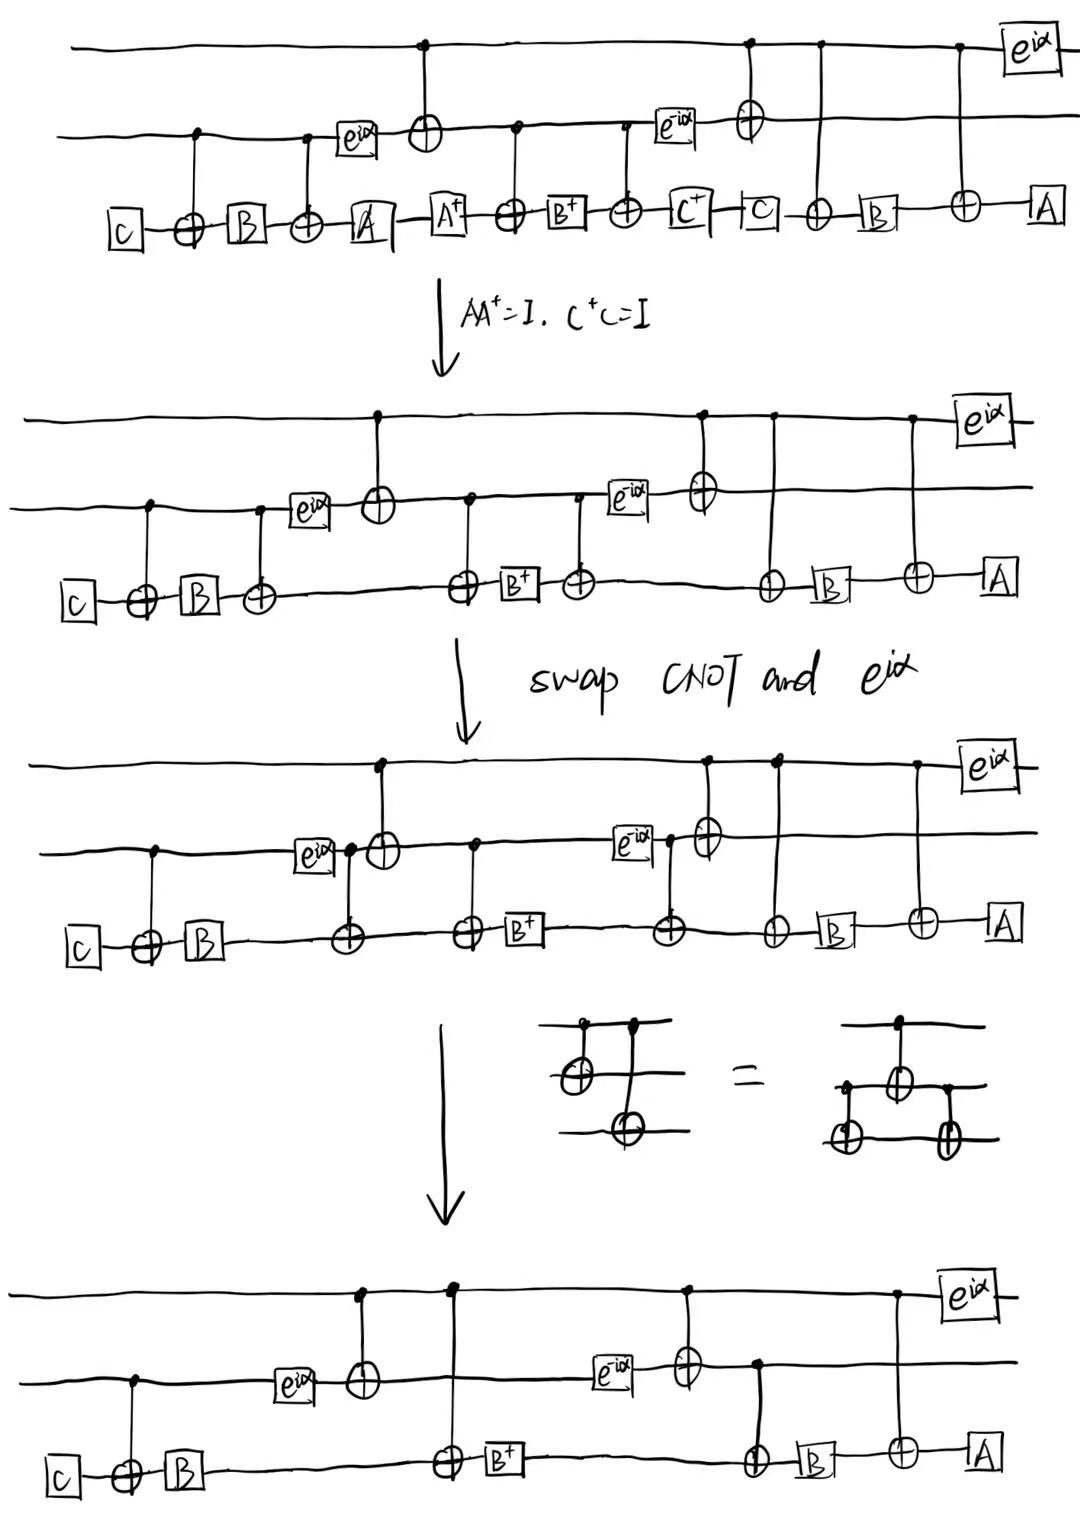
\includegraphics[width=0.8\textwidth]{figures/4-22.jpg}
    \caption{}
    \label{}
\end{figure}